\chapter{Introducción}
\thispagestyle{empty}


\section{Marco temático} \label{sec:\thesection}
\subsection{Esculturas cinéticas}
\subsubsection{Definición}
Las esculturas cinéticas (kinetic sculpture en inglés) son estructuras tridimensionales en donde el movimiento es una parte fundamental del conjunto. Para lograr el efecto de movimiento en el espacio estos sistemas se construyen con partes móviles que pueden cambiar de posición ya sea naturalmente por acción del viento, como se ve en la figura \ref{fig:1.1}, o de manera forzada.
% https://www.youtube.com/watch?v=D2HF-1xjpP8

\begin{figure}[!ht]
	\centering
	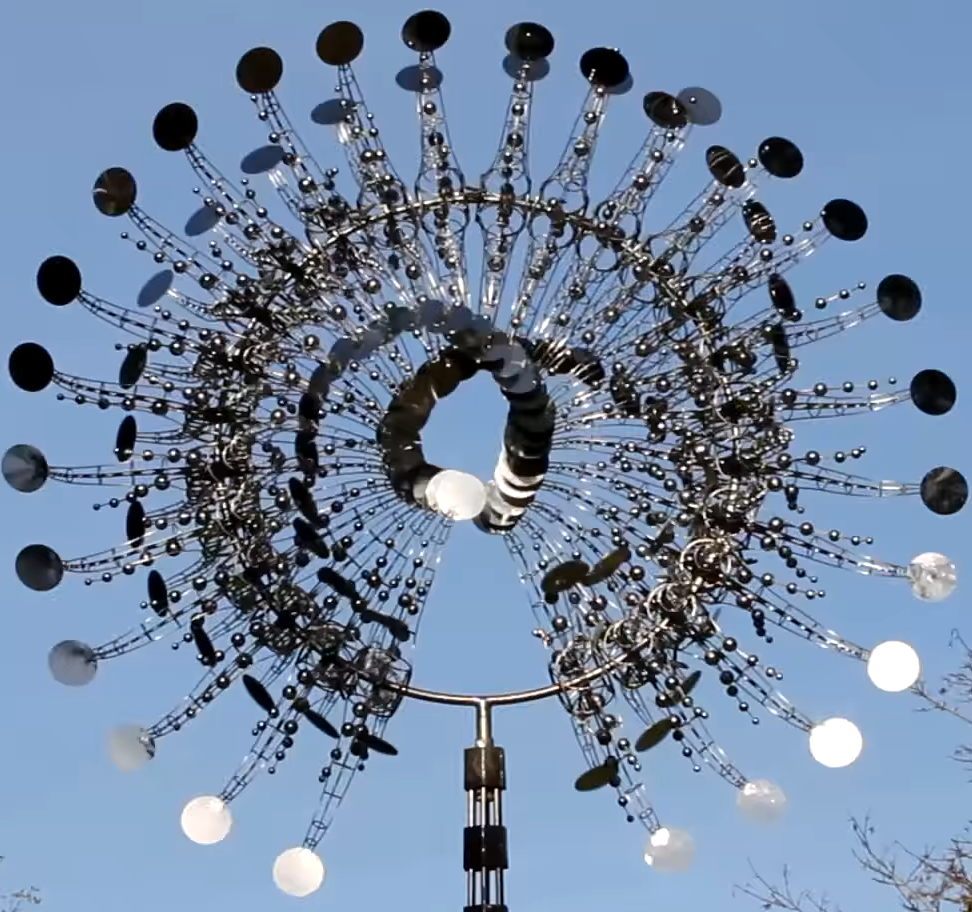
\includegraphics[width=10cm,scale=1]{resources/1_1-kinSculp.png}
	\caption{ Ejemplo de escultura cinética movida por aire, por Anthony Howe. Fuente:  \href{https://www.youtube.com/watch?v=N-1LpikCSR4}{LINK al video} }
	\label{fig:\thefigure}
\end{figure}

\newpage
\subsubsection{Aplicaciones y estado actual del arte}
Al ser obras que caen dentro del campo artístico suelen presentarse en museos y utilizarse para fines decorativos ya sea en parques o eventos. Sin embargo, el nivel de ingeniería y diseño que algunas de ellas requieren las tornan un interesante desafío intelectual y creativo.

Las aplicaciones puntuales de estructuras cinéticas a las que se hará foco en este informe, debido a la naturaleza del proyecto final, son aquellas en donde el efecto espacial se logra a través del movimiento en el eje vertical de objetos esféricos mediante motores. 

Un ejemplo de aplicación de estas características se puede ver en la figura \ref{fig:1.2}. Allí se muestra una escultura presentada en el Museo de BMW, en Munich, Alemania, en donde 714 esféras metálicas son coordinadas para formas figuras como olas, gotas, y hasta la silueta de un auto.

\begin{figure}[!ht]
	\centering
	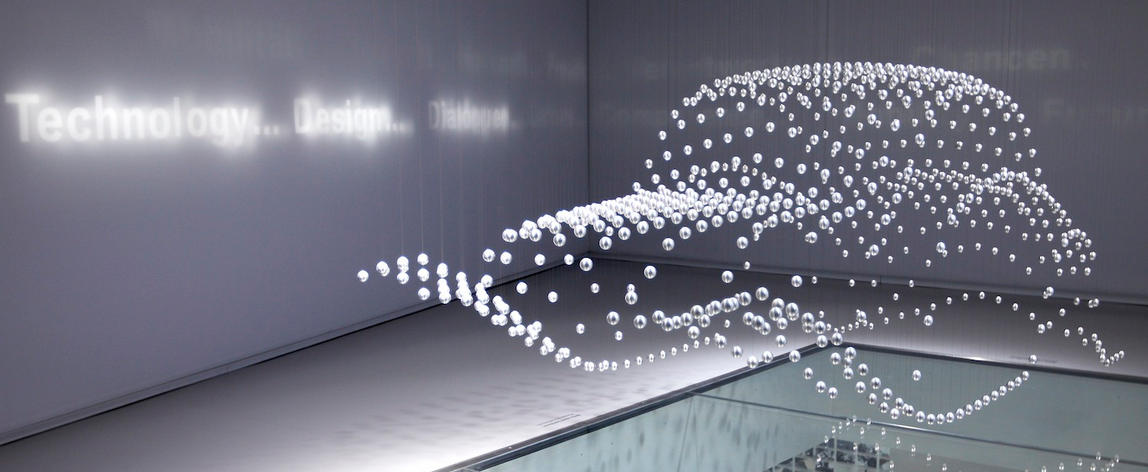
\includegraphics[width=15cm,scale=1]{resources/1_2-kinSculp.png}
	\caption{ Escultura cinética en el museo BMW. Fuente: \href{https://www.youtube.com/watch?v=HVhVClFMg6Y}{LINK al video} }
	\label{fig:\thefigure}
\end{figure}

Otro ejemplo de aplicación se puede ver en la figura \ref{fig:1.3}, en una obra presentada por la empresa Build Up en un centro comercial en Fukuoka, Japón. Allí se instalaron 1000 luminarias esféricas RGB dispuestas en una matriz de 25x40 para generar figuras tridimensionales como planos y gausseanas, entre otras. En este caso los efectos espaciales se logran coordinando el movimiento de cada esfera independientemente, cada una manejada por un equipo motorizado.
\begin{figure}[!ht]
	\centering
	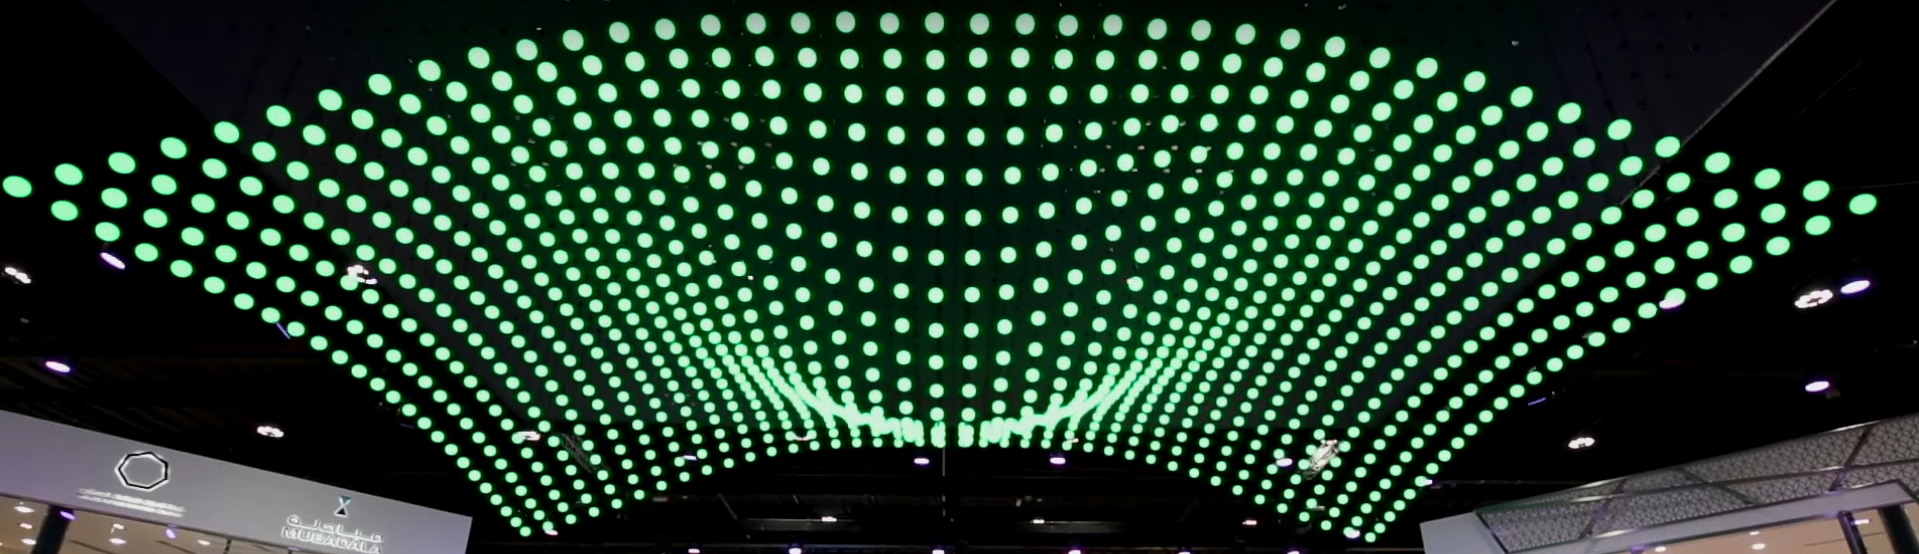
\includegraphics[width=15cm,scale=1]{resources/1_3-kinSculp.png}
	\caption{ Escultura cinética por parte de Build Up. Fuente: \href{https://www.youtube.com/watch?v=ICixCazf6-k}{LINK al video} }
	\label{fig:\thefigure}
\end{figure}

%\newpage


\subsection{Sistemas de iluminación} 
\subsubsection{Equipos de luces}
En cualquier espectáculo o evento la iluminación es una parte vital del show, y a medida que estos fueron evolucionando también lo hicieron los equipos de luces. Partiendo de aparatos fijos en donde solo se podía variar la intensidad de luz, se pueden conseguir hoy en día dispositivos complejos con decenas de parámetros controlables.\\
Un notable ejemplo es el \href{http://preworks.at/index.php/en/products/led-automated-luminairies/shapeshifter}{Shapeshifter}, figura \ref{fig:1.4}, que cuenta con 7 módulos leds que pueden ser manejados independientemente.

\begin{figure}[!ht]
	\centering
	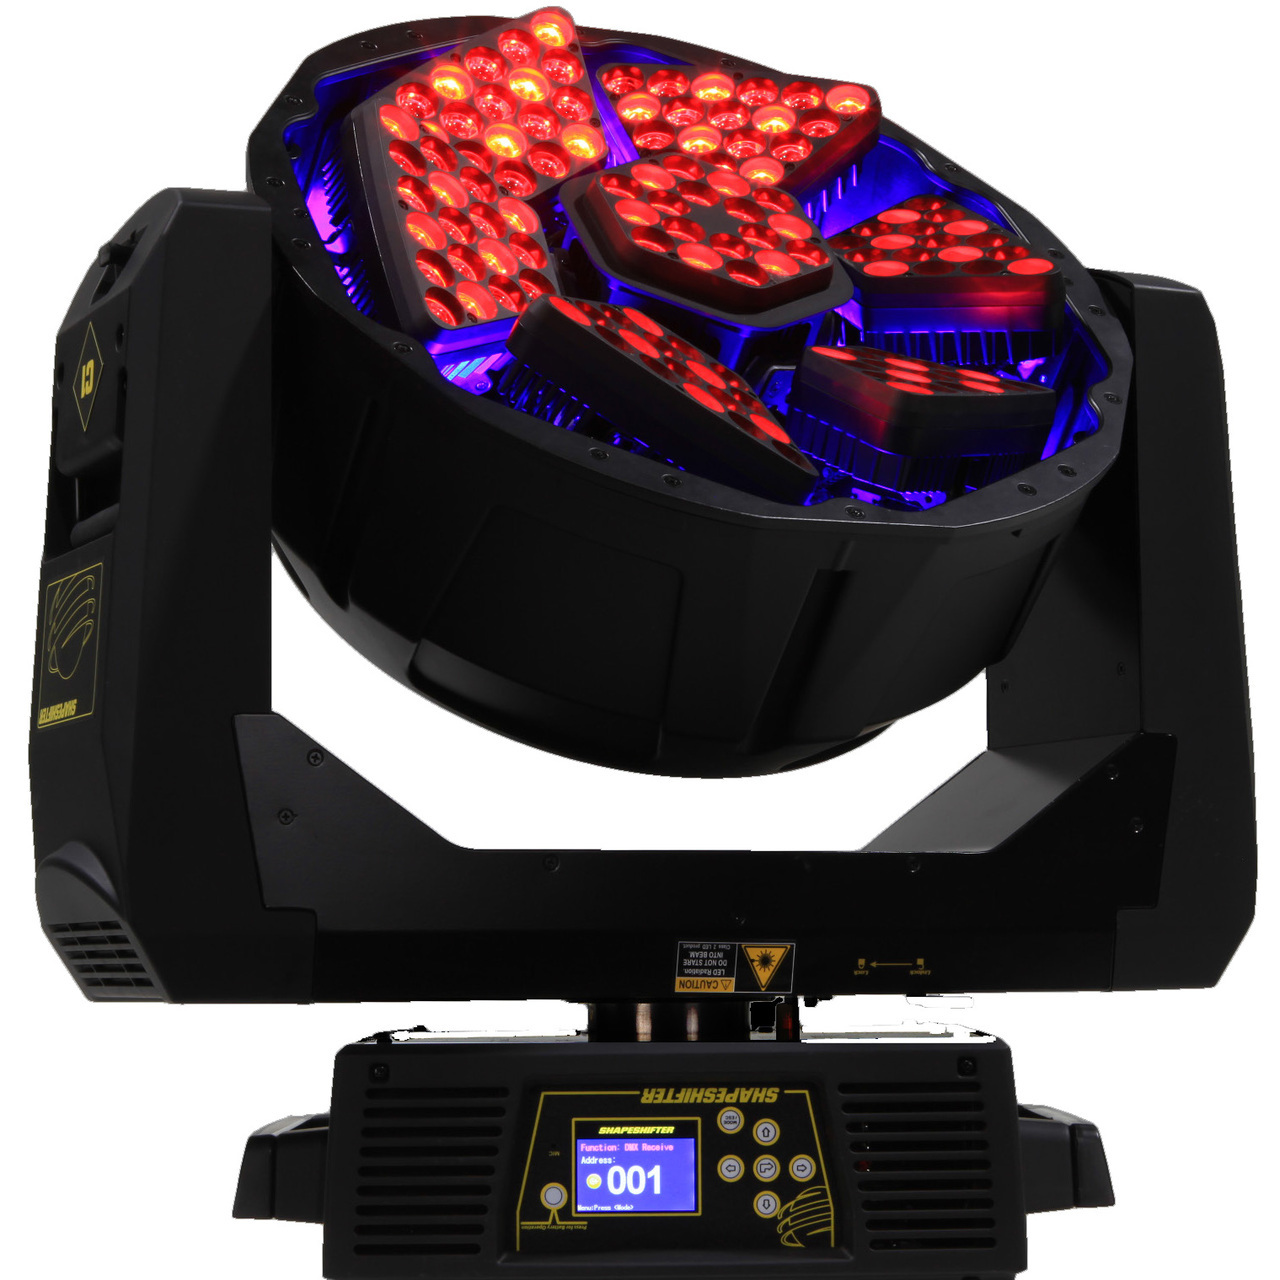
\includegraphics[width=7cm,scale=1]{resources/1_4-shapeshifter.jpg}
	\caption{Shapeshifter, de High End Systems. Fuente: \href{https://www.youtube.com/watch?v=LIIE3zZscYY}{LINK al video} }
	\label{fig:\thefigure}
\end{figure}

En el caso del sistema visto en la figura \ref{fig:1.3}, los parámetros controlables de los equipos son la posición, velocidad y colores de cada esfera.

\subsubsection{Consolas de control de luminaria}
Para controlar los sistemas de luces es necesario utilizar unas consolas especiales. Estas se comunican con las luminarias utilizando el estándar \textbf{DMX} y le indican a cada equipo el valor de sus parámetros en todo momento.

La manera más común para generar un efectos es indicando la progresión de uno o más parámetros desde un tiempo inicial a uno final. Al cambio de los parámetros entre 2 instantes de tiempo se las llama \textit{cues}, o entradas, y cuyo conjunto forma los efectos. \\
Dentro de las consolas que hay en el mercado para este tipo de control de equipos se pueden destacar las \href{https://www.highend.com/products/consoles}{consolas hog 4} de High End Systems, como la que se muestra en la figura \ref{fig:1.5}.

Otra manera generarlos es a partir de equipos y softwares, como el \href{https://www.madrix.com/}{Madrix}, que tienen la capacidad de convertir videos a variaciones de parámetros, lo cual lo hace especialmente útil cuando se quieren crear \href{https://www.youtube.com/watch?v=mdbl5ks7Nu0}{efectos lumínicos complejos}.


\begin{figure}[!ht]
	\centering
	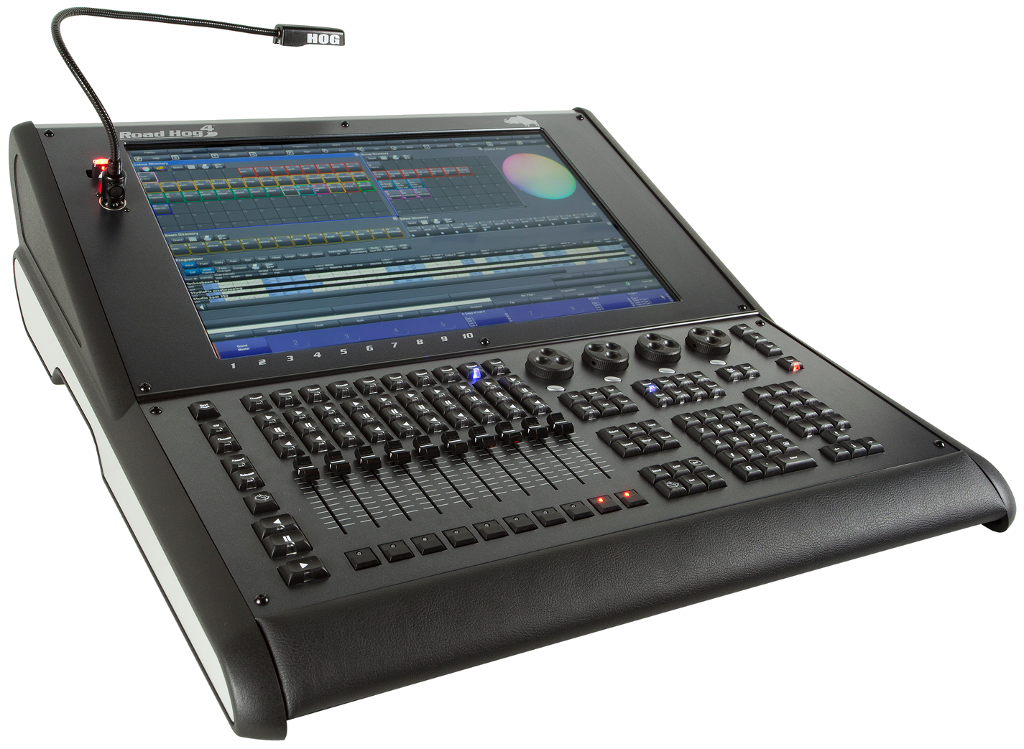
\includegraphics[width=10cm,scale=1]{resources/1_5-consolaHOG.png}
	\caption{Consola Hog4, de High End Systems. Fuente: \href{https://www.highend.com/products/consoles}{LINK a la imágen}}
	\label{fig:\thefigure}
\end{figure}

\newpage
\section{DMX} \label{sec:\thesection}
\subsection{Definición e historia}
DMX, de \textit{Digital MultipleX}, es un estándar de comunicación digital ámpliamente utilizado para el control de sistemas de iluminación. 

El estándar DMX512, donde 512 significa que se envían 512 piezas de información, fue creado por la \textit{United States Institute for Theatre Technology} (USITT) en 1986 y transformado en DMX512/1990 tras una revisión de la USITT. En 1998 la \textit{Entertainment Services and Technology Association} (ESTA) cuadró DMX dentro de los estándares ANSI, modificación que fue aprovada por el instituto (ANSI) en 2004. Finalmente, en 2008 DMX tuvo una nueva revisión y se llegó a la versión actual llamada "E1.11 – 2008, USITT DMX512-A", o simplemente DMX512-A. A pesar de esto, el nombre comúnmente conocido del estándar es simplemente DMX, aunque no es indistinto ya que hay diferencia de compatibilidad entre las diferentes versiones.


\subsection{Capa física}
\subsubsection{Cableado y conectores}
DMX empléa el estándar EIA-485 como capa física, por lo que emplea por lo menos 3 lineas; A, B y C, en donde A y B es por los datos son transmidos, y C es masa. Los conectores utilizados son los XLR, tanto de 5 como de 3 pines. Un ejemplo del cable se puede ver en la figura \ref{fig:1.6} \\

\begin{figure}[!ht]
	\centering
	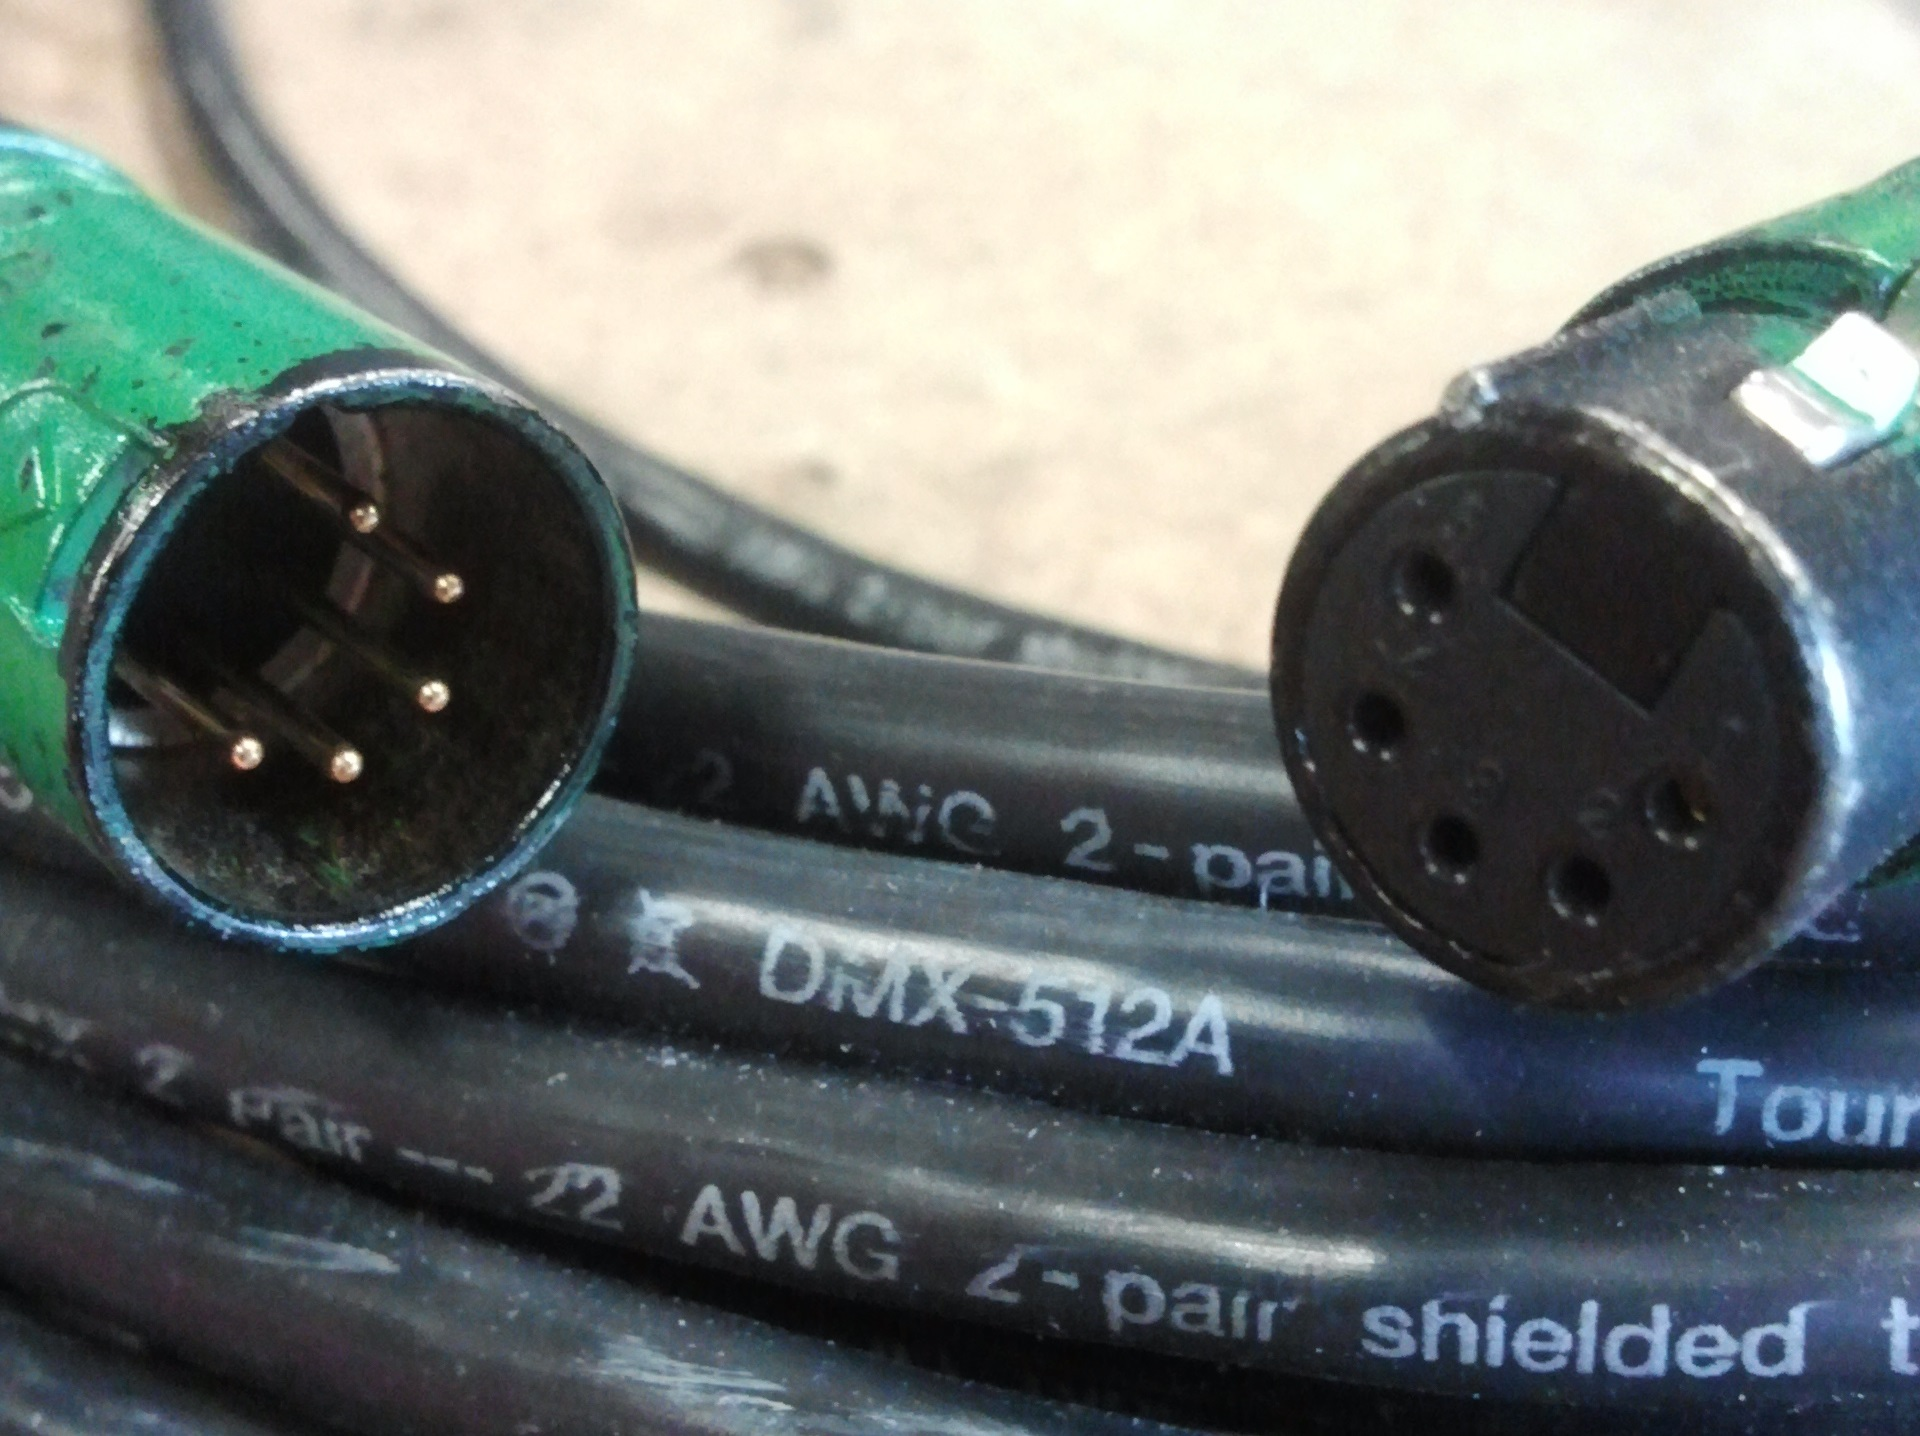
\includegraphics[width=8cm,scale=1]{resources/1_6-cableDMX.jpg}
	\caption{Cable DMX con conector XLR5. Fuente: wikipedia}
	\label{fig:\thefigure}
\end{figure}

\subsubsection{Topología}
La red de DMX consiste en un maestro y varios esclavos, conectados con una topología de bus multidrop (MDB) con nodos conectados entre sí, lo que normalmente se denomina como topología \textit{daisy chain}. En otras palabras, todos los equipos a controlar tienen una entrada y una salida conectadas entre sí, de manera tal de que se puede conectar un equipo y apartir de este equipo conectar el siguiente, y así sucesivente, como se ve en la figura \ref{fig:1.7}. Esto permite que el conexionado sea simple y que la red pueda ser fácilmente extendida.

\begin{figure}[!ht]
	\centering
	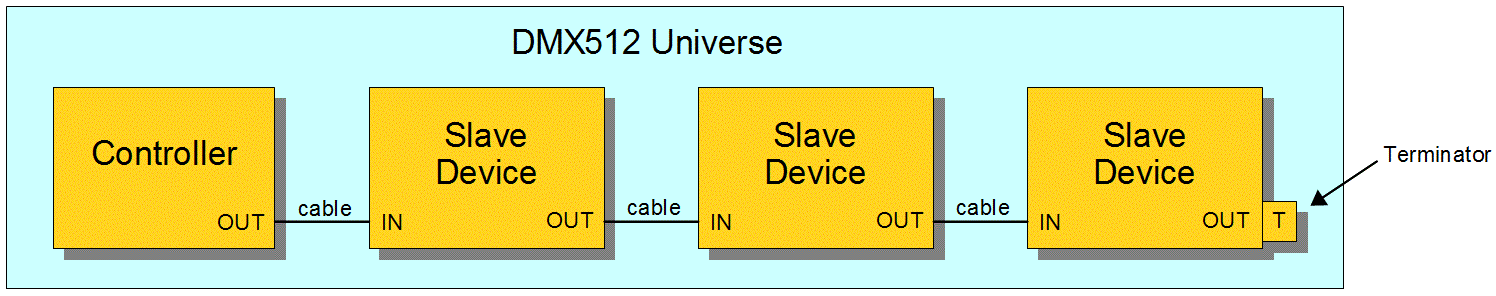
\includegraphics[width=15cm,scale=1]{resources/1_7-topologiaDMX.png}
	\caption{Conexionado en una red DMX. Fuente: wikipedia}
	\label{fig:\thefigure}
\end{figure}

\subsubsection{Señal}
La señal de DMX es de tipo diferencial, como es indicado en EIA-485, de 5 Volts de pico, y los datos se envían asincrónicamente de manera serie con una tasa de transmisión de 250Kbits por segundo que equivale a una duración de bit de 4\(\mu \)s.


\subsection{Capa de enlace de datos}
\subsubsection{Subcapa de control de enlace lógico}
La trama DMX, visible en la figura \ref{fig:1.8} consta de las siguientes partes:
%Fuentes: Fhttp://www.dmx512-online.com/packt.html 

\begin{itemize}
	\item \textbf{Idle} y \textbf{MTBP} (Mark Time Between Packets): estado de HIGH en la linea que indica la ausencia de señal de DMX. En caso de que se supere el tiempo máximo de 1 segundo sin datos, se considera que hubo una pérdida en la conexión.
	\item \textbf{Break}: estado de LOW en la línea utilizado para separar las tramas entre sí.
	\item \textbf{MAB} (Mark After Break): estado en HIGH enviado luego de un Break. Este estado suele traer problemas de compatibilidad ya que fue cambiado de una duración de 4\(\mu \)s a 8\(\mu \)s en la versión de DMX512 de 1990.
	\item \textbf{Slots}: son datos con formato 8N2 (un bit de start (LOW), 8 bits de datos, 2 bits de stop (HIGH) y sin paridad), y pueden ser:
	\begin{itemize}
		\item \textbf{SC} (Start Code): es el Slot 0, enviado luego de un MAB, para indicar el principio del payload. Todos los bits de datos equivalen a LOW en este estado.
		\item \textbf{Channels}: contienen la información que quiere ser enviada a los equipos de DMX. El conjunto de los 8 bits de datos pueden tomar un valor de 0 a 255. En total pueden haber un máximo de 512 canales enviados.
	\end{itemize}
	\item \textbf{MTBF} (Mark Time Between Frames): estado opcional de HIGH en la linea que puede agregarse antes del bit de start de cada canal.
\end{itemize}


\begin{table}[!ht]
	\begin{center}
		\begin{tabular}{|c|c|c|c|}
			\hline
			\rowcolor{OODlightblue}
			\textbf{Señal} & \textbf{Mínima} & \textbf{Máxima} & \textbf{Típica} \\
			\hline \hline
			Idle/MTBP & 0 & 1 seg & No especificada \\
			Break & 88\(\mu \)s & 1seg & 88\(\mu \)s\\
			MAB & - & - & 8\(\mu \)s \\
			Bit & - & - & 1/250KHz = 4\(\mu \)s \\
			Slot (11 bits) & - & - & 44\(\mu \)s \\
			MTBF & 0 & 1 seg & No especificada \\
			\hline
		\end{tabular}
	\end{center}
	\caption{Duración de las señales que componen la trama de DMX}
	\label{table:\thetable}
\end{table}

\begin{figure}[!ht]
	\centering
	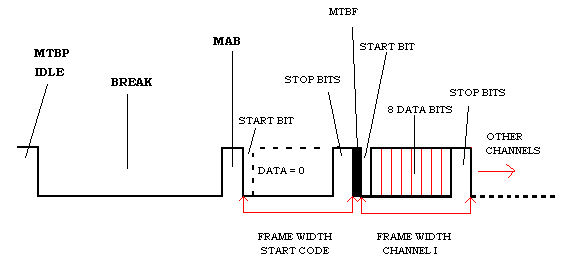
\includegraphics[width=15cm,scale=1]{resources/1_8-tramaDMX.png}
	\caption{Formato de la trama DMX. Fuente: \href{http://www.dmx512-online.com/packt.html}{LINK}}
	\label{fig:\thefigure}
\end{figure}

A cada trama con 512 canales se la llama "universo de DMX". Si se necesitan enviar más de 512 canales se utilizan más universos.

\subsubsection{Subcapa de control de acceso al medio}
DMX no implemente ningún mecanismo de control de acceso al medio debido a que el único transmisor es la red es el maestro y todos los esclavos reciben la misma información.

\section{Updown} \label{sec:\thesection}
\subsection{Definición}
El \textbf{Updown}, que se puede ver en la figura \ref{fig:1.9}, es básicamente una grúa que sube y baja una carga conforme a comandos recibidos por una equipo que utilice el protocolo DMX, como puede ser una consola de control de luminaria. La distancia máxima a la que la carga puede bajar es de 4 metros.

Este producto fue concebido en \textbf{Blackout}, una empresa productora y proveedora de tecnología cuyo objetivo es generar contenido audiovisual para grandes eventos. Blackout tomó interés en esculturas cinéticas como la de la figura \ref{fig:1.3} pero se encontró con el problema que el costo de importación de los equipos utilizados para tales fines, sumado a su precio unitario, era muy elevado. Por este motivo, decidió comenzar el desarrollo de un producto propio y nacional para alcanzar su objetivo.\\

\begin{figure}[!ht]
	\centering
	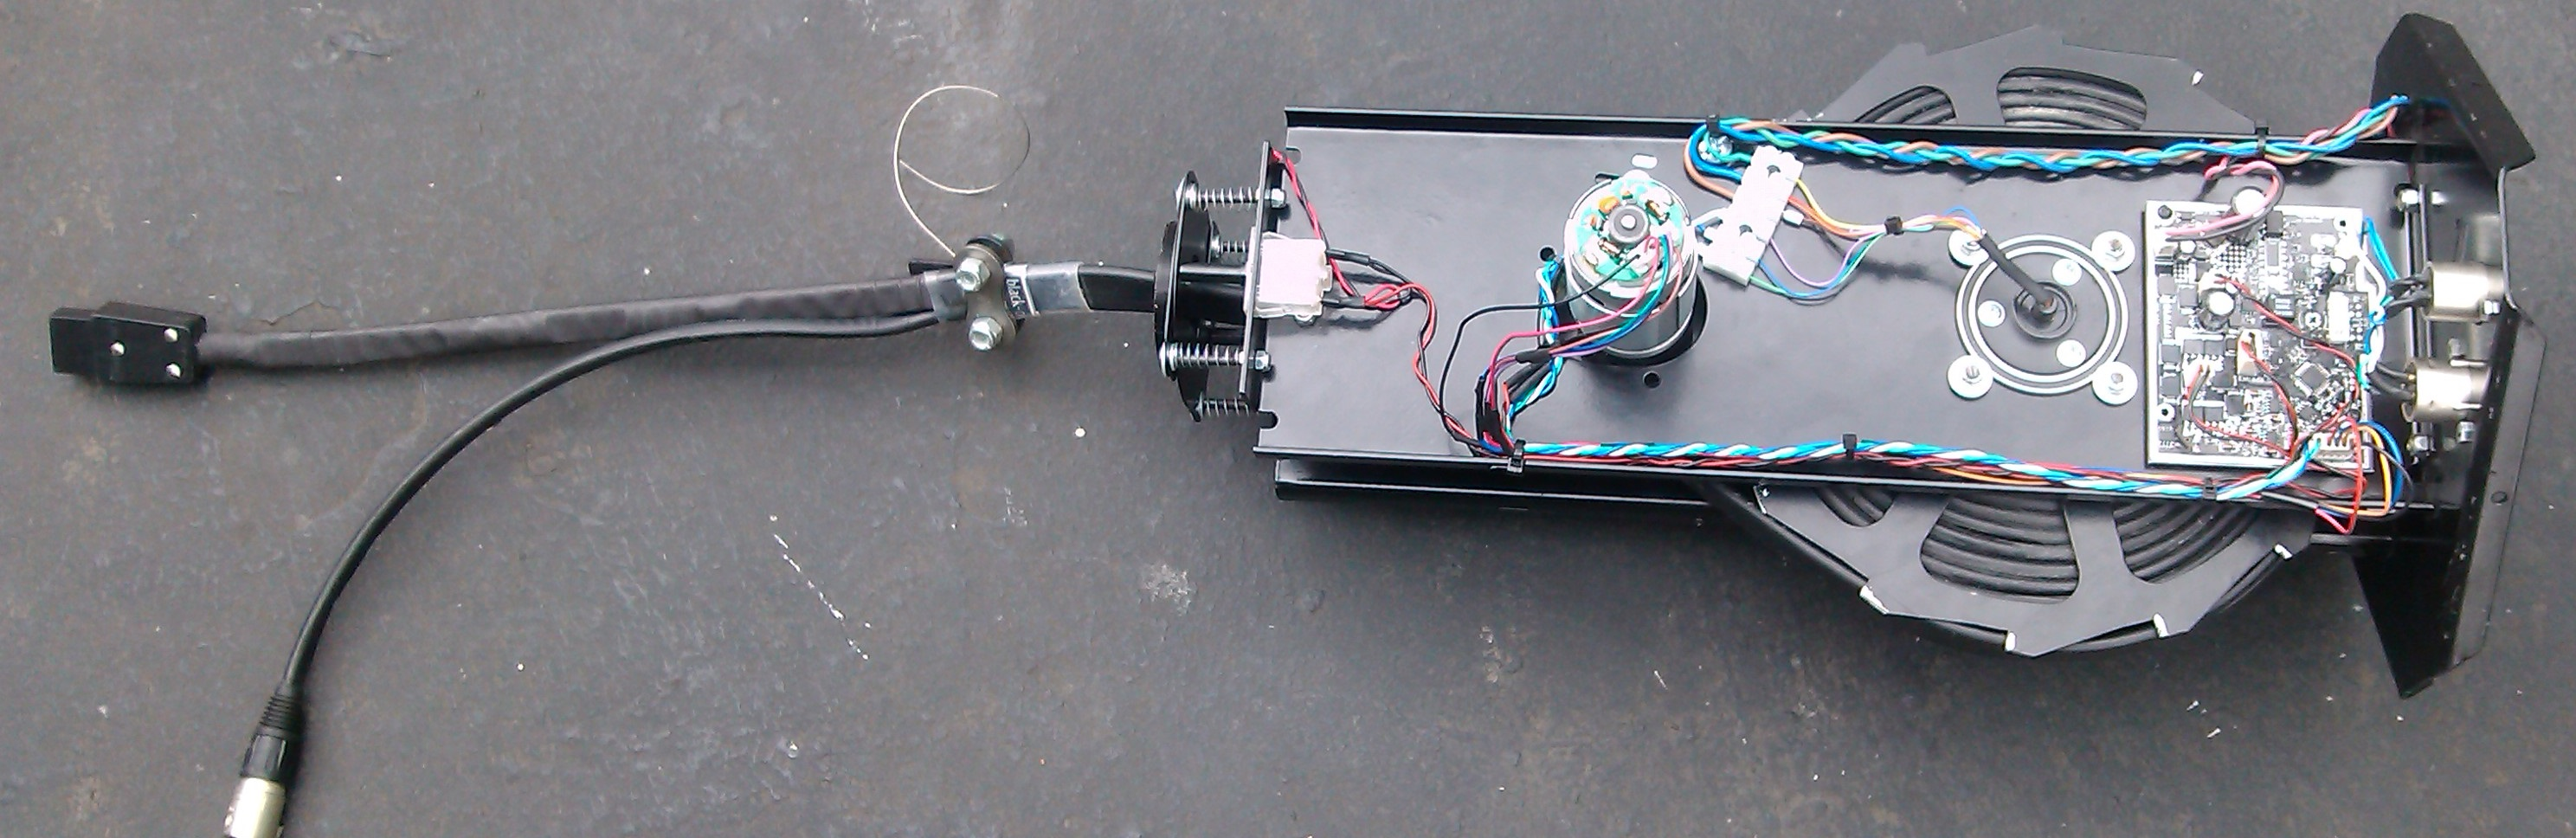
\includegraphics[width=15cm,scale=1]{resources/1_9-updown.jpg}
	\caption{Imágen del Updown, desarrollado por la empresa Blackout}
	\label{fig:\thefigure}
\end{figure}
\newpage
\subsection{Descripción del sistema}

En la figura \ref{fig:1.10} se presenta el diagrama general del equipo updown. Allí se pueden identificar todos elementos electrónicos y mecánicos que conforman el sistema, los agentes externos del sistema, y la comunicación entre ellos.

\begin{figure}[!ht]
	\centering
	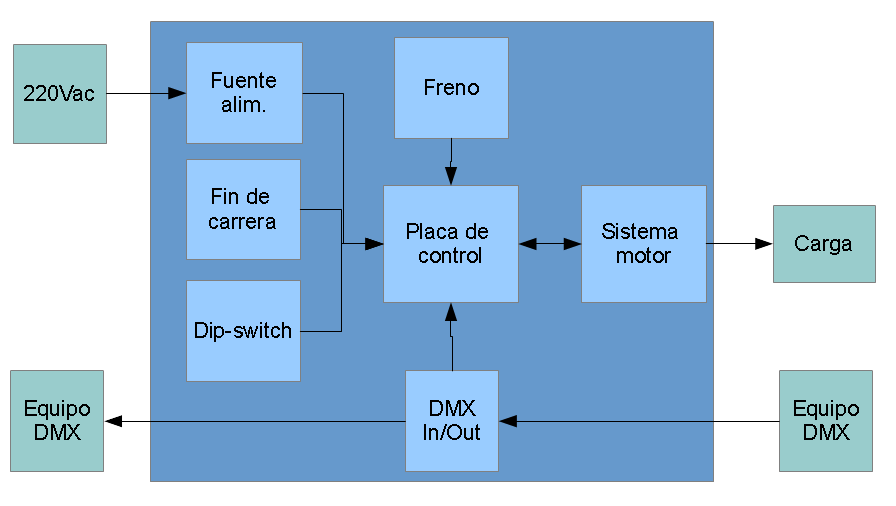
\includegraphics[width=15cm,scale=1]{resources/1_10-diagramaBasicoUpdown.png}
	\caption{Diagrama conceptual del equipo Updown}
	\label{fig:\thefigure}
\end{figure}

\subsubsection{Fuente de alimentación}
La fuente de alimentación es la encargada de proveer la potencia necesaria para el funcionamiento del sistema motor, y de placa de control junto con sus periféricos. Esto lo logra convirtiendo la tensión de red de 220Vac a una señal continua de 24Vcc, entregando 4.5A máximo.

\subsubsection{Entrada y salida DMX}
La señal DMX proveniente del master de la red, otro Updown, o cualquier otro equipo esclavo dentro del mismo universo DMX ingresa al sistema para ser procesada por la placa de control. Su función es indicarle al equipo la referencia de posición y velocidad, y los parámetros que correspondan a la carga.\\
Además, para cumplir con el estándar DMX, la señal de entrada se replica mediante un puente a una salida para que otro equipo pueda ser conectado a la red.

\subsubsection{Dip-switch}
El dipswitch consta con varios divisores resistivos, 10 switchs y un led indicador. Su función es seleccionar el canal inicial de DMX con el que el equipo trabajará.

\subsubsection{Freno}
El freno consta de una bobina, desactivada por defecto, que mueve una varilla metálica que traba el carrete que contiene la polea. Al activar la bobina la varilla libera al carrete, permitiendo el libre movimiento de la carga.

\subsubsection{Fin de carrera}
El fin de carrera consta de un par de pulsadores en la base del equipo. Eventos como enrollar completamente la polea activa alguno de los pulsadores, dandole aviso a la placa de control.

\subsubsection{Sistema motor}
El elemento principal del sistema motor es un motor de continua de 24V con un encoder AB en su eje. Este motor mueve un carrete en donde se enrolla el cable que sostiene la carga, que tiene un peso de 3Kg. El carrete, llamado disco, tiene unas marcas que son sensadas por un encoder en la placa de control para tener una segunda referencia de posición. La dirección de giro del motor se selecciona a través de un puente H.

\begin{figure}[!ht]
	\centering
	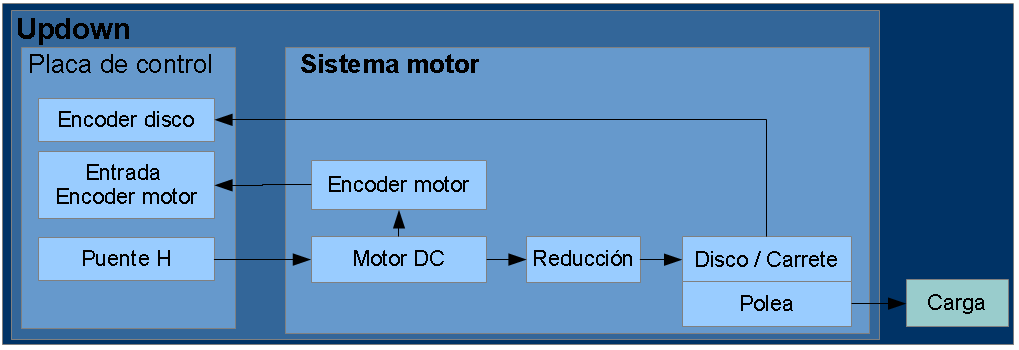
\includegraphics[width=15cm,scale=1]{resources/1_11-diagramaSistemaMotor.png}
	\caption{Diagrama del sistema motor}
	\label{fig:\thefigure}
\end{figure}

\subsubsection{Placa de control}
La placa de control contiene electrónica para el manejo de las entradas y salidas del sistema, y un controlador para manejar todos los periféricos siguiendo la lógica deseada.\\

\begin{figure}[!ht]
	\centering
	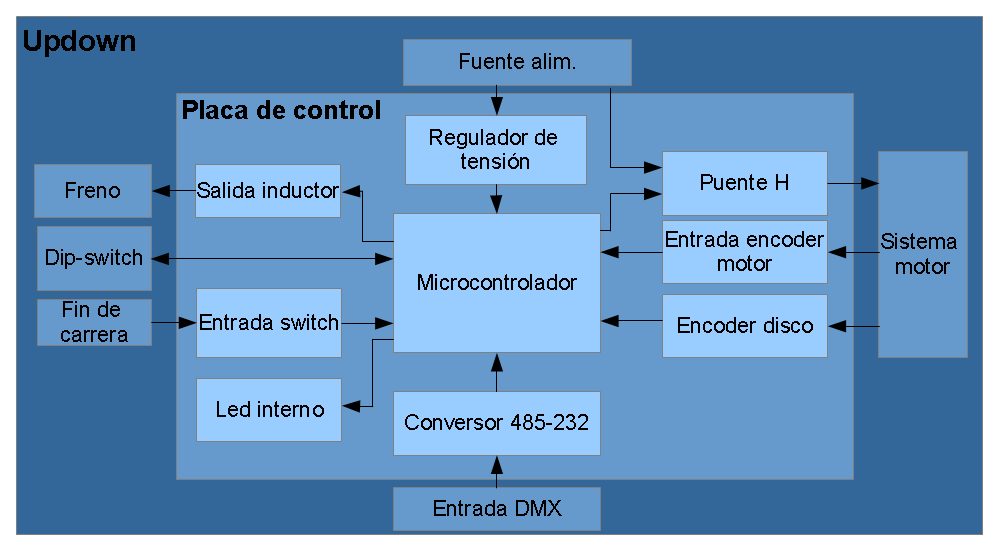
\includegraphics[width=15cm,scale=1]{resources/1_12-diagramaPlacaControl.png}
	\caption{Diagrama de la placa de control y su interacción con el hardware externo}
	\label{fig:\thefigure}
\end{figure}


\subsection{Resumen de entradas y salidas del sistema}
\subsubsection{Entradas} 
Señal de DMX, Fin de carrera, Dip-switch, Encoder AB de disco, Encoder AB de motor.\\
\subsubsection{Salidas}
Freno, Motor, Led interno (led indicador de la Placa de control), Led externo (led indicador del Dipswitch), Puente H.

\newpage
\section{Justificación del proyecto} \label{sec:\thesection}
Durante el desarrollo del updown la empresa se dió cuenta que con los recursos que contaban, tiempo en particular, no podían concretar los requerimientos que buscaban que el updown tuviera. 

Por este motivo, Blackout se vió en la necesidad de buscar a alguien externo a la empresa para darle fin al proyecto, lo que presentó la oportunidad de realizar el trabajo de concluir el desarrollo del equipo, que es en lo que este proyecto final se basa.

\section{Objetivos} \label{sec:\thesection}
El objetivo del proyecto es que el Updown suba y baje una carga de 3Kg, siguiendo las referencias de posición y velocidad dadas por un master DMX. Además, debe contar con ciertos mecanísmos de detección y manejo de errores para hacer que el producto sea seguro. También se tiene que terminar el desarrollo del dipswitch.\\
Como la mayoría del hardware del equipo resuelto las tareas a complir para terminar el producto, y dar por concluido el proyecto, se pueden resumur en los siguientes 4 requisitos:

\subsection{REQ-01}
Contar con el software necesario para el manejo de todas las entradas y salidas del sistema.
\subsection{REQ-02}
Lograr que las cargas manejadas por los equipos se muevan a la velocidad y posición indicadas mediante una consola DMX. Adicionalmente, las rampas de aceleración y desaceleración no deben ser bruscas ya que si varios equipos frenan violentamente podría causar daños estructurales en el lugar donde estén colgados.
\subsection{REQ-03}
Manejar errores y excepciones de hardware para lograr que el producto sea seguro, siendo que será instalado en eventos con un alto nivel de concurrencia.\\
Dentro de estos errores se eneucntran: corte de cadena, pérdida de señal DMX y accionamiento indebido del fin de carrera.
\subsection{REQ-04}
Concluir el desarrollo del dipswitch.

%\subsection{Productos que compiten en el mercado}
%El equipos más conocido empleado para estas aplicaciones es el \href{http://www.eastsunlite.com/p31.html}{OrbisFly}, de \href{https://www.kinetic-lights.com/}{Kinetic Lights}. Estos dispositivos de orígen Chino trabajan con una esfera RGB de peso estándar de 1Kg, aunque soporta un peso máximo de 2Kg, que puede descender hasta 9 metros. Dispone de un display LCD y botoneras para el testeo y configuración el equipo\\





